% Author: PokMan Ho pok.ho19@imperial.ac.uk
% Script: plot.tex
% Desc: R plot section
% Input: none
% Output: none
% Arguments: 0
% Date: Jan 2020

\documentclass[../note.tex]{subfiles} %% use packages & commands as this main file

\begin{document}

\section{Plots}
R is built by statisticians for data, so plotting in R is easy, flexible and powerful (as long as you know how to tweak parameters with correct grammar, which make the previous statement =trash).  So below are some probably handy commands from the base R environment, hopefully assisting you to make R work for you.

\subsection{Plot by group, data in wide format}
For plotting number-number plots (plotting y$\sim$x, z$\sim$x, ... together), this \href{http://www.datasciencemadesimple.com/matplot-in-r/}{code} from ``graphics" package\autocite{Rcore} is particularly useful.

To demonstrate it, we need a suitable wide table format numeric data as below:
\begin{code}
b<-seq(1e3)\\
\# get a number sequence starting from 1, having 1e3 number of elements\\\\
b<-data.frame("time"=b, "y1"=runif(length(b))*10, "y2"=rnorm(length(b), mean = 10, sd = 5), "y3"=sample(c(0,2,4), length(b), replace = T))\\
\# define a data.frame with content in one go\\
\# incorporate the sequence into data frame ("time" col)\\
\# generate random numbers with elements same with length of the sequence ("y1" col)\\
\# same number of elements, from a normal distribution ("y2" col)\\
\# sample that number of elements from the given pool with element replacement ("y3" col)
\end{code}
Then plot with
\begin{code}
matplot(x=b\$time, y=b[,-1], type="l", col = cbp, xlab = "time unit", ylab = "values", main="matplot demonstration")\\
\# x-axis\\
\# y-elements, columnwise excluding first column\\
\# line-type plot\\
\# line/point colour according to pre-defined colour-palette\\
\# manual set x-label\\
\# manual set y-label\\
\# manual set chart title\\\\

legend("topleft", legend = c("y1", "y2", "y3"), pch = rep(16,3), col = cbp)\\
\# use a pre-defined legend position\\
\# group labels\\
\# dot style indicating group in the graph\\
\# colour of dots indicating for the groups
\end{code}
And the plot look like this:\\
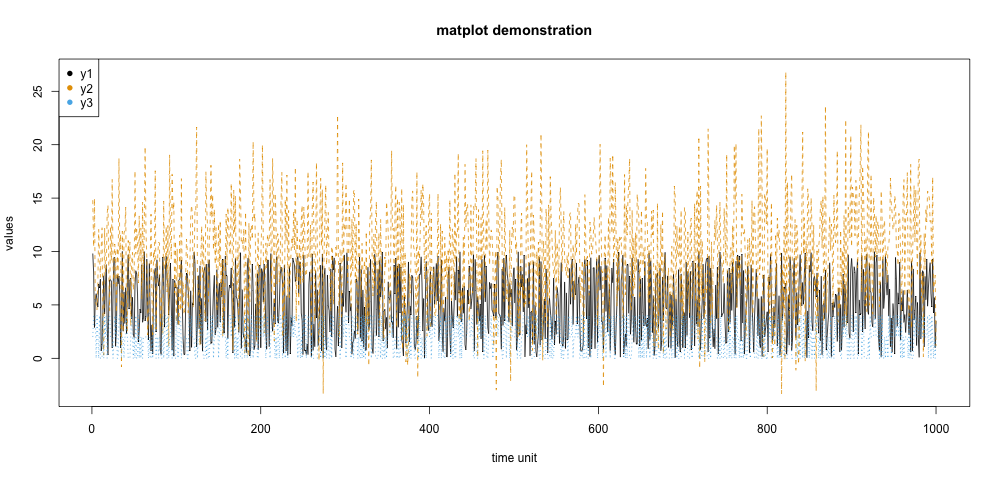
\includegraphics[width=.9\linewidth]{../graph/matplot.png}

\subsection{Legend position out of plot area}
Using the same matplot, we can tweak a bit and make the legend \href{https://stackoverflow.com/questions/3932038/plot-a-legend-outside-of-the-plotting-area-in-base-graphics}{outside} of the plot area
\begin{code}
par(mar=c(5.1, 4.1, 4.1, 8.1), xpd=TRUE)\\\\
matplot(x=b\$time, y=b[,-1], type="l", col = cbp, xlab = "time unit", ylab = "values", main="matplot demonstration")\\\\
legend("topright", inset=c(-.05,0), legend = c("y1", "y2", "y3"), pch = rep(16,3), col = cbp)\\
\# inset: x-shift, y-shift (positive as right and up)
\end{code}
And the plot look like this:\\
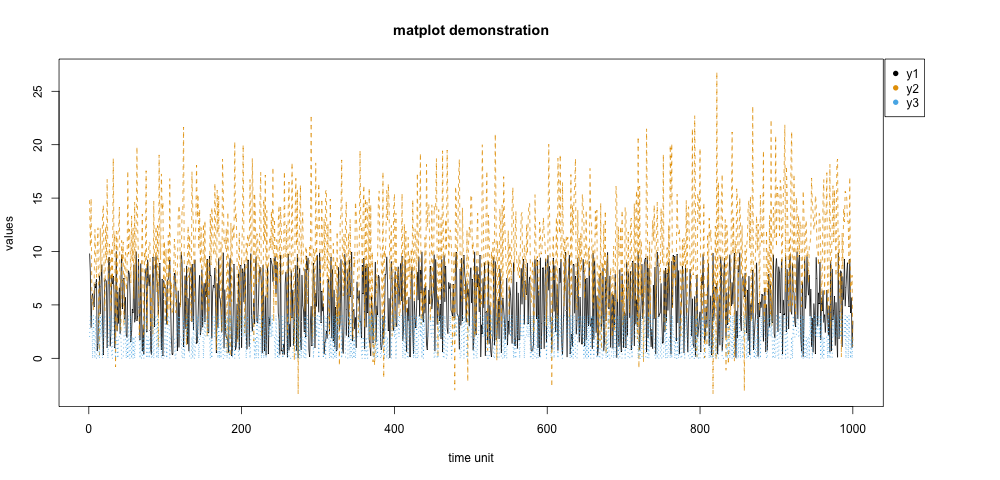
\includegraphics[width=.9\linewidth]{../graph/matplot1.png}

\end{document}